\subsection{The U-boot bootloader}

\begin{frame}{U-Boot}
  \begin{columns}
    \column{0.7\textwidth}
      U-Boot is a typical free software project
      \begin{itemize}
      \item License: GPLv2 (same as Linux)
      \item Freely available at \url{https://www.denx.de/wiki/U-Boot}
      \item Documentation available at
        \url{https://u-boot.readthedocs.io/en/latest/}
      \item The latest development source code is available in a Git
        repository:
        \url{https://gitlab.denx.de/u-boot/u-boot}
      \item Development and discussions happen around an open mailing-list
        \url{https://lists.denx.de/pipermail/u-boot/}
      \item Follows a regular release schedule. Every 2 or 3 months,
        a new version is released. Versions are named \code{YYYY.MM}.
      \end{itemize}
    \column{0.3\textwidth}
    \includegraphics[width=\textwidth]{slides/sysdev-bootloaders-u-boot/u-boot-logo.pdf}\\
    {\tiny \href{https://en.wikipedia.org/wiki/Das_U-Boot\#/media/File:U-Boot_Logo.svg}{Image source}}
  \end{columns}
\end{frame}

\begin{frame}{Where to get U-Boot from?}
  \begin{itemize}
  \item {\bf Ideal:} your platform is supported directly by {\bf
      upstream} U-Boot
    \begin{itemize}
    \item Best quality $\rightarrow$ code reviewed and approved by the community
    \item Long-term maintenance
    \item Use directly U-Boot from
      \url{https://gitlab.denx.de/u-boot/u-boot} Git repository
    \end{itemize}
  \item {\bf Less ideal:} use a {\bf fork} of U-Boot by your silicon
    vendor, system-on-module vendor or board vendor
    \begin{itemize}
    \item Generally older, does not follow all upstream U-Boot updates
    \item Changes not reviewed by the community $\rightarrow$ quality
      is often dubious
    \item Check your HW vendor documentation/SDK
    \end{itemize}
  \item If designing your own custom board
    \begin{itemize}
    \item You will have to port U-Boot
    \item If good support for your SoC in upstream U-Boot
      $\rightarrow$ use upstream U-Boot
    \item If not $\rightarrow$ use the U-Boot fork from your SoC
      vendor
    \end{itemize}
  \end{itemize}
\end{frame}

\begin{frame}{U-Boot configuration}
  \begin{itemize}
  \item Configuration system based on {\em kconfig} from the Linux
    kernel
  \item The \projdir{u-boot}{configs} directory contains configuration
    files for supported boards or platforms
    \begin{itemize}
    \item There may be a single configuration supporting multiple
      boards based on the same processor
    \item The configuration files defines all relevant options: CPU
      type, drivers needed, U-Boot features to compile in
    \item Examples:
      \begin{itemize}
      \item \projfile{u-boot}{configs/stm32mp15_basic_defconfig}
      \item \projfile{u-boot}{configs/stm32mp15_trusted_defconfig}
      \end{itemize}
    \end{itemize}
  \item Note: migration to {\em kconfig} is still on-going
    \begin{itemize}
    \item Not all boards have been converted to the new configuration
      system.
    \item Many boards still have a combination of configuration
      settings in \projfile{u-boot}{include/configs/} header files,
      and configuration settings in \code{defconfig} files
    \end{itemize}
  \end{itemize}
\end{frame}

\begin{frame}[fragile]
  \frametitle{U-Boot configuration file: {\tt stm32mp15\_trusted\_defconfig}}
  \begin{block}{}
    {\tiny
\begin{verbatim}
CONFIG_ARM=y
CONFIG_ARCH_STM32MP=y
CONFIG_TFABOOT=y
CONFIG_SYS_MALLOC_F_LEN=0x3000
CONFIG_ENV_OFFSET=0x280000
CONFIG_ENV_SECT_SIZE=0x40000
CONFIG_DEFAULT_DEVICE_TREE="stm32mp157c-ev1"
[..]
CONFIG_CMD_ADTIMG=y
CONFIG_CMD_ERASEENV=y
CONFIG_CMD_NVEDIT_EFI=y
CONFIG_CMD_MEMINFO=y
CONFIG_CMD_MEMTEST=y
CONFIG_CMD_UNZIP=y
CONFIG_CMD_ADC=y
CONFIG_CMD_CLK=y
CONFIG_CMD_DFU=y
CONFIG_CMD_FUSE=y
CONFIG_CMD_GPIO=y
[...]
CONFIG_SPI=y
CONFIG_DM_SPI=y
CONFIG_STM32_QSPI=y
CONFIG_STM32_SPI=y
[...]
\end{verbatim}
    }
  \end{block}
  See the full file: \projfile{u-boot}{configs/stm32mp15_trusted_defconfig}
\end{frame}

\begin{frame}[fragile]{U-Boot configuration}
  \begin{columns}
    \column{0.6\textwidth}
    \begin{itemize}
    \item U-Boot must be configured before being compiled
    \item Configuration stored in a \code{.config} file
    \item Load a pre-defined configuration
\begin{verbatim}
$ make BOARDNAME_defconfig
\end{verbatim}
      Where \code{BOARDNAME} is the name of a configuration, as
      visible in the \projdir{u-boot}{configs} directory.
    \item You can then run \code{make menuconfig} to further customize
      U-Boot's configuration.
    \end{itemize}
    \column{0.4\textwidth}
    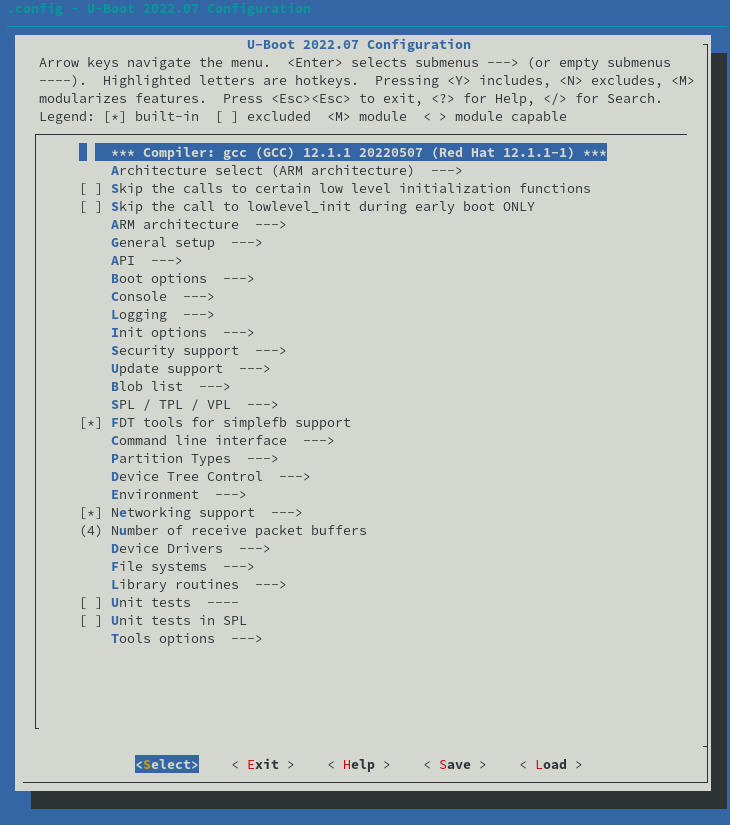
\includegraphics[width=\textwidth]{slides/sysdev-bootloaders-u-boot/uboot-menuconfig.png}
  \end{columns}
\end{frame}

\begin{frame}[fragile]{U-Boot compilation}
  \begin{itemize}
  \item The path to the cross-compiler must be specified in the
    \code{CROSS_COMPILE} variable
  \item \code{CROSS_COMPILE} contains the prefix common to all
    cross-compilation tools, e.g \code{arm-linux-}
  \item Common to add the cross-compiler location in \code{PATH} to
    keep the \code{CROSS_COMPILE} value short
\begin{verbatim}
$ export PATH=/path/to/toolchain/bin:$PATH
$ make CROSS_COMPILE=arm-linux-
\end{verbatim}
  \item The main result is a \code{u-boot.bin} file, which is the
    U-Boot image.
  \item Depending on your specific platform, or what storage device
    you're booting from (NAND or MMC), there may be other specialized
    images: \code{u-boot.img}, \code{u-boot.kwb}...
  \end{itemize}
\end{frame}

\begin{frame}{Concept of U-Boot SPL}
  \begin{itemize}
  \item To meet the need of a two-stage boot process, U-Boot has the
    concept of {\em U-Boot SPL}
  \item SPL = {\em Secondary Program Loader}
  \item The SPL is a stripped-down version of U-Boot, made small
    enough to meet the size constraints of a first stage bootloader
  \item Configured through {\em menuconfig}, one can define the subset
    of drivers to include
  \item No U-Boot shell/commands: the behavior is hardcoded in C code
  \item For some platforms: TPL, {\em Tertiary Program Loader}, an
    even more minimal first stage bootloader to do TPL
    $\rightarrow$ SPL $\rightarrow$ main U-Boot.
  \end{itemize}
\end{frame}

\begin{frame}{Device Tree in U-Boot}
  \begin{itemize}
  \item The {\em Device Tree} is a data structure that describes the
    topology of the hardware
  \item Allows software to known which hardware peripherals are
    available and how they are connected to the system
  \item Initially mainly used by Linux, now also used by U-Boot,
    Barebox, TF-A, etc.
  \item Used by U-Boot on many platforms, but not all!
  \item Device Tree files located in \code{arch/ARCH/dts}
  \item One \code{.dts} for each board: need to create one if you
    build a custom board
  \item U-Boot {\em defconfigs} usually specify a default Device Tree,
    but it can be overridden using the \code{DEVICE_TREE} variable
  \item More details on the {\em Device Tree} later in this course.
  \end{itemize}
\end{frame}

\begin{frame}[fragile]{U-Boot build example: TI AM335x BeagleBoneBlack wireless}
  \begin{itemize}
  \item One {\em defconfig} file suitable for all AM335x platforms:
    \projfile{u-boot}{configs/am335x_evm_defconfig}
    \begin{itemize}
    \item Yes its name looks like it supports only the EVM (EValuation
      Module) board
    \item Contains \code{CONFIG_DEFAULT_DEVICE_TREE="am335x-evm"}
      $\rightarrow$ uses
      \projfile{u-boot}{arch/arm/dts/am335x-evm.dts} by default
    \end{itemize}
  \item One {\em Device Tree} file describing the BeagleBoneBlack
    Wireless:
    \projfile{u-boot}{arch/arm/dts/am335x-boneblack-wireless.dts}
  \item Configure and build U-Boot
\begin{verbatim}
$ export PATH=/path/to/toolchain/bin:$PATH
$ make am335x_evm_defconfig
$ make DEVICE_TREE=am335x-boneblack-wireless CROSS_COMPILE=arm-linux-
\end{verbatim}
  \item Produces:
    \begin{itemize}
    \item \code{MLO}, the SPL, first-stage bootloader. Called MLO ({\em
    Mmc LOad}) as required on TI platforms.
    \item \code{u-boot.img}, full U-Boot, second-stage bootloader
    \end{itemize}
  \end{itemize}
\end{frame}

\begin{frame}{Installing U-Boot in flash (NAND or eMMC)}
  Different possibilities depending on the hardware:
  \begin{enumerate}
  \item The ROM code provides some kind of specific boot monitor with
    which you can communicate through the serial port or USB using a
    specific protocol, to flash U-Boot.
  \item The CPU boots first on removable media (SD card) before
    booting from fixed media. In this case, boot from
    removable media to reflash a new version.
  \item U-Boot is already installed, and can be used to flash a new
    version of itself. If the new version of U-Boot doesn't work,
    you will have to reflash it through another method (it is always
    possible through an external SD card).
  \item The board provides a JTAG interface, which allows to write to
    the flash memory remotely, without any system running on the
    board.
  \end{enumerate}
\end{frame}

\begin{frame}[fragile]{U-boot shell prompt}
  \begin{columns}
    \column{0.5\textwidth}
    \begin{itemize}
    \item Connect the target to the host through a serial console.
    \item Power-up the board. On the serial console, you should
      see U-Boot starting up.
    \item The U-Boot shell offers a set of commands.
    \item The U-Boot shell is not a Linux shell: commands are
      completely different from Linux ones.
    \end{itemize}
    \column{0.5\textwidth}
    \begin{block}{}
      {\tiny
\begin{verbatim}
U-Boot SPL 2022.01 (Mar 31 2022 - 14:58:17 +0200)
Trying to boot from MMC1

U-Boot 2022.01 (Mar 31 2022 - 14:58:17 +0200)

CPU  : AM335X-GP rev 2.1
Model: TI AM335x BeagleBone Black
DRAM:  512 MiB
WDT:   Started wdt@44e35000 with servicing (60s timeout)
NAND:  0 MiB
MMC:   OMAP SD/MMC: 0, OMAP SD/MMC: 1
Loading Environment from FAT... OK
Net:   Could not get PHY for ethernet@4a100000: addr 0
eth2: ethernet@4a100000, eth3: usb_ether [PRIME]
Hit any key to stop autoboot:  0
=>
\end{verbatim}
      }
    \end{block}
  \end{columns}
\end{frame}

\begin{frame}[fragile]{U-Boot {\tt help} command}
  \begin{columns}
    \column{0.5\textwidth}
    \begin{itemize}
    \item \code{help} command to list all available commands
    \item The set of available commands depend on the U-Boot
      configuration
      \begin{itemize}
      \item Many \code{CONFIG_CMD_*} options to enable commands at
        compile time
      \item See {\em Command line interface} submenu in
        \code{menuconfig}
      \end{itemize}
    \item \code{help <command>} for the complete help of one command
    \end{itemize}
    \column{0.5\textwidth}
    \begin{block}{}
      {\tiny
\begin{verbatim}
STM32MP> help
?         - alias for 'help'
adc       - ADC sub-system
adtimg    - manipulate dtb/dtbo Android image
base      - print or set address offset
[...]
usb       - USB sub-system
[...]

STM32MP> help usb
usb - USB sub-system

Usage:
usb start - start (scan) USB controller
usb reset - reset (rescan) USB controller
usb stop [f] - stop USB [f]=force stop
usb tree - show USB device tree
usb info [dev] - show available USB devices
[...]
\end{verbatim}
      }
    \end{block}
  \end{columns}
\end{frame}

\begin{frame}[fragile]{U-Boot information commands}

  \begin{columns}
    \column{0.5\textwidth}
    \begin{block}{Version details: \code{version}}
      {\tiny
\begin{verbatim}
=> version
U-Boot 2020.04 (May 26 2020 - 16:05:43 +0200)
arm-linux-gcc (crosstool-NG 1.24.0.105_5659366) 9.2.0
GNU ld (crosstool-NG 1.24.0.105_5659366) 2.34
\end{verbatim}
      }
    \end{block}

    \begin{block}{NAND flash information: \code{nand info}}
      {\tiny
\begin{verbatim}
=> nand info
Device 0: nand0, sector size 128 KiB
  Page size       2048 b
  OOB size          64 b
  Erase size    131072 b
  subpagesize     2048 b
  options     0x40004200
  bbt options 0x00008000
\end{verbatim}
      }
    \end{block}

    \begin{block}{MMC information: \code{mmc info}}
      {\tiny
\begin{verbatim}
=> mmc info
Device: STM32 SD/MMC
Manufacturer ID: 3
[...]
Capacity: 14.8 GiB
Bus Width: 4-bit
\end{verbatim}
      }
    \end{block}

    \column{0.5\textwidth}

    \begin{block}{Board information: \code{bdinfo}}
      {\tiny
\begin{verbatim}
=> bdinfo
boot_params = 0x00000000
DRAM bank   = 0x00000000
-> start    = 0xc0000000
-> size     = 0x20000000
flashstart  = 0x00000000
flashsize   = 0x00000000
flashoffset = 0x00000000
baudrate    = 115200 bps
relocaddr   = 0xddb21000
reloc off   = 0x1da21000
[...]
fdt_blob    = 0xdbb01950
new_fdt     = 0xdbb01950
fdt_size    = 0x0001d540
Video       = display-controller@5a001000 inactive
[...]
\end{verbatim}
      }
    \end{block}

    {\scriptsize
      \begin{itemize}
      \item DRAM starts at \code{0xc0000000}, for a size of 512~MB
        (\code{0x20000000}).
      \item The end of the memory is used by U-Boot itself:
        \code{relocaddr} is the location of U-Boot in RAM.
      \end{itemize}
    }
  \end{columns}
\end{frame}

\begin{frame}{Concept of U-Boot environment}
  \begin{itemize}
  \item A significant part of the U-Boot configuration happens at
    compile time: \code{menuconfig}
  \item U-Boot also has runtime configuration, through the concept of
    {\em environment variables}
  \item Environment variables are key/value pairs
    \begin{itemize}
    \item Some specific environment variables impact the behavior of
      different U-Boot commands
    \item Additional custom environment variables can be added, and
      used in {\em scripts}
    \end{itemize}
  \item U-Boot environment variables are stored and modified in RAM
  \item U-Boot has a default environment built into its binary
    \begin{itemize}
    \item used when no other environment is found
    \item defined in the configuration
    \item the default environment is sometimes quite complex in some
      existing configurations
    \end{itemize}
  \item The environment can be persistently stored in non-volatile
    storage
  \end{itemize}
\end{frame}

\begin{frame}{U-Boot environment persistent storage}
  \begin{columns}
    \column{0.5\textwidth}
    Depending on the configuration, the U-Boot environment can be:
    \begin{itemize}
    \item At a fixed offset in NAND flash
    \item At a fixed offset on MMC or USB storage, before the
      beginning of the first partition.
    \item In a file on a FAT or ext4 partition
    \item In a UBI volume
    \item Not stored at all, only the built-in environment in the
      U-Boot binary is used
    \end{itemize}
    \column{0.5\textwidth}
    \includegraphics[width=\textwidth]{slides/sysdev-bootloaders-u-boot/u-boot-environment-configuration.png}\\
    \vspace{0.3cm}
    \tiny U-Boot environment configuration menu
  \end{columns}
\end{frame}

\begin{frame}{U-Boot environment commands}
  \begin{itemize}
    \item \code{printenv}\\
      Shows all variables
    \item \code{printenv <variable-name>}\\
      Shows the value of a variable
    \item \code{setenv <variable-name> <variable-value>}\\
      Changes the value of a variable or defines a new one, only in RAM
    \item \code{editenv <variable-name>}\\
      Interactively edits the value of a variable, only in RAM
    \item After an \code{editenv} or \code{setenv}, changes in the
      environment are lost if they are not saved persistently
    \item \code{saveenv}\\
      Saves the current state of the environment to storage for persistence.
    \item \code{env} command, with many sub-commands: \code{env
        default}, \code{env info}, \code{env erase}, \code{env set},
      \code{env save}, etc.
  \end{itemize}
\end{frame}

\begin{frame}[fragile]{U-Boot environment commands example}
  \begin{block}{}
\small
\begin{verbatim}
=> printenv
baudrate=19200
ethaddr=00:40:95:36:35:33
netmask=255.255.255.0
ipaddr=10.0.0.11
serverip=10.0.0.1
stdin=serial
stdout=serial
stderr=serial
=> setenv serverip 10.0.0.100
=> printenv serverip
serverip=10.0.0.100
=> saveenv
\end{verbatim}
\end{block}
\end{frame}

\begin{frame}{U-Boot memory allocation}
  \begin{itemize}
  \item Many commands in U-Boot loading data into memory, or using
    data from memory, expect a RAM address as argument
  \item No built-in memory allocation mechanism $\rightarrow$ up to
    the user to know usable memory areas to load/use data
  \item Use the output of \code{bdinfo} to know the start address and
    size of RAM
  \item Avoid the end of the RAM, which is used by the U-Boot code and
    dynamic memory allocations
  \item Not the best part of the U-Boot design, sadly
  \end{itemize}
\end{frame}

\begin{frame}{U-Boot memory manipulation commands}
  \begin{itemize}
  \item Commands to inspect or modify any memory location, useful for
    debugging, poking into hardware registers, etc.
  \item Addresses manipulated in U-Boot are directly physical
    addresses
  \item Memory display\\
    \codewithhash{md [.b, .w, .l, .q] address [\# of objects]}
  \item Memory write\\
    \code{mw [.b, .w, .l, .q] address value [count]}
  \item Memory modify (modify memory contents interactively starting from address)\\
    \code{mm [.b, .w, .l, .q] address}
  \end{itemize}
\end{frame}

\begin{frame}{U-Boot raw storage commands}
  U-Boot can manipulate raw storage devices:
  \begin{columns}
    \column{0.6\textwidth}
    \begin{itemize}
    \item NAND flash
      \begin{itemize}
      \item \code{nand info}
      \item \code{nand read addr off|partition size}
      \item \code{nand erase off size}
      \item \code{nand write addr off|partition size}
      \item More: \code{help nand}
      \end{itemize}
    \item MMC
      \begin{itemize}
      \item \code{mmc info}
      \item \codewithhash{mmc read addr blk\# cnt}
      \item \codewithhash{mmc write addr blk\# cnt}
      \item \code{mmc part} to show partition table
      \item \code{mmc dev} to show/set current MMC device
      \item More: \code{help mmc}
      \end{itemize}
    \end{itemize}
    \column{0.4\textwidth}
    \vfill
    \begin{itemize}
    \item USB storage
      \begin{itemize}
      \item \code{usb info}
      \item \codewithhash{usb read addr blk\# cnt}
      \item \codewithhash{usb write addr blk\# cnt}
      \item \code{usb part}
      \item \code{usb dev}
      \item More: \code{help usb}
      \end{itemize}
    \end{itemize}
  \end{columns}
  \vspace{0.2cm}
  Note: \code{addr} are addresses in RAM where data is stored
\end{frame}

\begin{frame}[fragile]{U-Boot commands example}
  \begin{columns}
    \column{0.5\textwidth}
    \begin{block}{List partitions on MMC}
      {\tiny
\begin{verbatim}
STM32MP> mmc part
Partition Map for MMC device 0  --   Partition Type: EFI

Part    Start LBA       End LBA         Name
        Attributes
        Type GUID
        Partition GUID
  1     0x00000022      0x000001d3      "fsbl1"
        attrs:  0x0000000000000000
        type:   0fc63daf-8483-4772-8e79-3d69d8477de4
        type:   linux
        guid:   72c63477-c475-4cf7-988e-b763bce4604e
  2     0x000001d4      0x00000385      "fsbl2"
        attrs:  0x0000000000000000
        type:   0fc63daf-8483-4772-8e79-3d69d8477de4
        type:   linux
        guid:   66d616db-de56-4a1e-9b13-9b1a5a6e360f
  3     0x00000386      0x00001385      "fip"
        attrs:  0x0000000000000000
        type:   0fc63daf-8483-4772-8e79-3d69d8477de4
        type:   linux
        guid:   6251ecf7-d985-4d81-a396-7a6b6fab8b7c
  [...]
\end{verbatim}
      }
    \end{block}
    \column{0.5\textwidth}

    \begin{block}{Read block 0x22 from MMC to RAM 0xc0000000}
      {\tiny
\begin{verbatim}
STM32MP> mmc read c0000000 22 1

MMC read: dev # 0, block # 34, count 1 ... 1 blocks read: OK
\end{verbatim}
      }
    \end{block}

    \begin{block}{Dump memory at 0xc00000000}
      {\tiny
\begin{verbatim}
STM32MP> md c0000000
c0000000: 324d5453 00000000 00000000 00000000  STM2............
c0000010: 00000000 00000000 00000000 00000000  ................
c0000020: 00000000 00000000 00000000 00000000  ................
c0000030: 00000000 00000000 00000000 00000000  ................
\end{verbatim}
      }
    \end{block}
  \end{columns}
\end{frame}

\begin{frame}{U-Boot filesystem storage commands}
  \begin{itemize}
  \item U-Boot has support for many filesystems
    \begin{itemize}
    \item The exact list of supported filesystems depends on the U-Boot
      configuration
    \end{itemize}
  \item Per-filesystem commands
    \begin{itemize}
    \item FAT: \code{fatinfo}, \code{fatls}, \code{fatsize},
      \code{fatload}, \code{fatwrite}
    \item ext2/3/4: \code{ext2ls}, \code{ext4ls}, \code{ext2load},
      \code{ext4load}, \code{ext4size}, \code{ext4write}
    \item Squashfs: \code{sqfsls}, \code{sqfsload}
    \end{itemize}
  \item ``New'' generic commands, working for all filesystem types
    \begin{itemize}
    \item Load a file: \code{load <interface> [<dev[:part]> [<addr> [<filename> [bytes [pos]]]]]}
    \item List files: \code{ls <interface> [<dev[:part]> [directory]]}
    \item Get the size of a file: \code{size <interface> <dev[:part]> <filename>}\\
	  (result stored in \code{filesize} environment variable)
    \item \code{interface}: \code{mmc}, \code{usb}
    \item \code{dev}: device number, \code{0} for first device, \code{1} for second device
    \item \code{part}: partition number
    \end{itemize}
  \end{itemize}
\end{frame}

\begin{frame}[fragile]{U-Boot filesystem command example}
  \begin{columns}
    \column{0.5\textwidth}
    \begin{block}{List files}
      {\tiny
\begin{verbatim}
STM32MP> ls mmc 0:4
<DIR>       1024 .
<DIR>       1024 ..
<DIR>      12288 lost+found
<DIR>       2048 bin
<DIR>       1024 boot
<DIR>       1024 dev
<DIR>       1024 etc
[...]

STM32MP> ls mmc 0:4 /etc
<DIR>       1024 .
<DIR>       1024 ..
             209 asound.conf
<DIR>       1024 fonts
             334 fstab
             347 group
[...]
\end{verbatim}
      }
    \end{block}

    \column{0.5\textwidth}
    \begin{block}{Load file}
      {\tiny
\begin{verbatim}
STM32MP> load mmc 0:4 c0000000 /etc/fstab
334 bytes read in 143 ms (2 KiB/s)
\end{verbatim}
      }
    \end{block}

    \begin{block}{Show file contents}
      {\tiny
\begin{verbatim}
STM32MP> md c0000000
c0000000: 663c2023 20656c69 74737973 093e6d65  # <file system>.
c0000010: 756f6d3c 7020746e 3c093e74 65707974  <mount pt>.<type
c0000020: 6f3c093e 6f697470 093e736e 6d75643c  >.<options>.<dum
c0000030: 3c093e70 73736170 642f0a3e 722f7665  p>.<pass>./dev/r
c0000040: 09746f6f 6509092f 09327478 6e2c7772  oot./..ext2.rw,n
[...]
\end{verbatim}
      }
    \end{block}
  \end{columns}
\end{frame}

\begin{frame}{U-Boot networking}
  \begin{itemize}
  \item Environment variables
    \begin{itemize}
    \item \code{ethaddr}: MAC address
    \item \code{ipaddr}: IP address of the board
    \item \code{serverip}: IP address of the server for network related commands
    \end{itemize}
  \item Important commands
    \begin{itemize}
    \item \code{ping}: ping a destination machine. Note: U-Boot is not
      an operating system with multitasking/interrupts, so ping from
      another machine to U-Boot cannot work.
    \item \code{tftp}: load a file using the TFTP protocol
    \item \code{dhcp}: get an IP address using DHCP
    \end{itemize}
  \end{itemize}
\end{frame}

\begin{frame}{TFTP}
  \begin{itemize}
  \item Network transfer from the development workstation to U-Boot
    on the target takes place through TFTP
    \begin{itemize}
    \item {\em Trivial File Transfer Protocol}
    \item Somewhat similar to FTP, but without authentication and over
      UDP
    \end{itemize}
  \item A TFTP server is needed on the development workstation
    \begin{itemize}
    \item \code{sudo apt install tftpd-hpa}
    \item All files in \code{/srv/tftp} are then visible through TFTP
    \item A TFTP client is available in the \code{tftp-hpa} package,
      for testing
    \end{itemize}
  \item A TFTP client is integrated into U-Boot
    \begin{itemize}
    \item Configure the \code{ipaddr}, \code{serverip}, and
      \code{ethaddr} environment variables
    \item Use \code{tftp <address> <filename>} to load file contents to
      the specified RAM address
    \item Example: \code{tftp 0x21000000 zImage}
    \end{itemize}
  \end{itemize}
\end{frame}

\begin{frame}{Scripts in environment variables}
  \begin{itemize}
  \item Environment variables can contain small scripts, to execute
    several commands and test the results of commands.
    \begin{itemize}
    \item Useful to automate booting or upgrade processes
    \item Several commands can be chained using the \code{;} operator
    \item Tests can be done using
      \code{if command ; then ... ; else ... ; fi}
    \item Scripts are executed using \code{run <variable-name>}
    \item You can reference other variables using
      \code{${variable-name}}
    \end{itemize}
  \item Examples
    \begin{itemize}
    \item \code{setenv bootcmd 'tftp 0x21000000 zImage; tftp 0x22000000 dtb; bootz 0x21000000 - 0x22000000'}
    \item \code{setenv mmc-boot 'if fatload mmc 0 80000000
      boot.ini; then source; else if fatload mmc 0 80000000 zImage;
      then run mmc-do-boot; fi; fi'}
  \end{itemize}
\end{itemize}
\end{frame}

\begin{frame}{U-Boot booting commands}
  \begin{itemize}
  \item Commands to boot a Linux kernel image
    \begin{itemize}
    \item \code{bootz} $\rightarrow$ boot an ARM32 \code{zImage}
    \item \code{booti} $\rightarrow$ boot an ARM64 or RISC-V \code{Image}
    \item \code{bootm} $\rightarrow$ boot a kernel image with U-Boot header
    \item \code{zboot} $\rightarrow$ boot an x86 \code{bzImage}
    \end{itemize}
  \item \code{bootz [addr [initrd[:size]] [fdt]]}
    \begin{itemize}
    \item \code{addr}: address of the kernel image in RAM
    \item \code{initrd}: address of the {\em initrd} or {\em initramfs}, if any. Otherwise, must pass \code{-}
    \item \code{fdt}: address of the {\em Device Tree} passed to the Linux kernel
    \end{itemize}
  \item Important environment variables
    \begin{itemize}
    \item \code{bootcmd}: list of commands executed automatically by
      U-Boot after the count down
    \item \code{bootargs}: Linux kernel command line
    \end{itemize}
  \end{itemize}
\end{frame}

\begin{frame}[fragile]{U-Boot booting example}
  \begin{block}{Load kernel image and Device Tree}
    {\tiny
\begin{verbatim}
STM32MP> ls mmc 0:4 /boot
<DIR>       1024 .
<DIR>       1024 ..
          117969 stm32mp157c-dk2.dtb
         7538376 zImage

STM32MP> load mmc 0:4 c2000000 /boot/zImage
7538376 bytes read in 463 ms (15.5 MiB/s)

STM32MP> load mmc 0:4 c4000000 /boot/stm32mp157c-dk2.dtb
117969 bytes read in 148 ms (778.3 KiB/s)
\end{verbatim}
    }
  \end{block}

  \begin{block}{Set kernel command line and boot}
    {\tiny
\begin{verbatim}
STM32MP> setenv bootargs root=/dev/mmcblk0p4 rootwait

STM32MP> bootz c2000000 - c4000000
Kernel image @ 0xc2000000 [ 0x000000 - 0x7306c8 ]
## Flattened Device Tree blob at c4000000
   Booting using the fdt blob at 0xc4000000
   Loading Device Tree to cffe0000, end cffffcd0 ... OK
[...]
\end{verbatim}
    }
  \end{block}
\end{frame}

\begin{frame}{FIT image}
  \begin{itemize}
  \item U-Boot has a concept of {\bf FIT} image
  \item FIT = {\em Flat Image Tree}
  \item Container format that allows to bundle multiple images into
    one
    \begin{itemize}
    \item Multiple kernel images
    \item Multiple Device Trees
    \item Multiple initramfs
    \item Any other image: FPGA bitstream, etc.
    \end{itemize}
  \item Interestingly, relies on the {\em Device Tree Compiler}
    \begin{itemize}
    \item \code{.its} file describe the contents of the image
    \item Device Tree Compiler compiles it into an \code{.itb}
    \end{itemize}
  \item U-Boot can load an \code{.itb} image and use its different
    elements
  \item \url{https://www.thegoodpenguin.co.uk/blog/u-boot-fit-image-overview/}
  \item \url{https://source.denx.de/u-boot/u-boot/-/tree/master/doc/uImage.FIT}
  \end{itemize}
\end{frame}

\begin{frame}{Generic Distro boot (1)}
  \begin{itemize}
  \item Each board/platform used to have its own U-Boot environment,
    with custom variables/commands
  \item Wish to standardize the behavior of bootloaders, including
    U-Boot
  \item {\em Generic Distro boot} concept
  \item If enabled, at boot time, U-Boot:
    \begin{itemize}
    \item Can be asked to locate a bootable partition (\code{part list} command),
          as defined by the bootable flag of the partition table
    \item With the \code{sysboot} command, will look for a
          \code{/extlinux/extlinux.conf} or \code{/boot/extlinux/extlinux.conf}
	  file describing how to boot, and will offer a prompt in the console
          to choose between available configurations.
    \item Once a configuration is selected, will load and boot the
          corresponding kernel, device tree and initramfs images.
    \item Example \code{bootcmd}:\\
          \code{part list mmc 0 -bootable bootpart; sysboot mmc 0:${bootpart} any}
    \end{itemize}
  \item \url{https://u-boot.readthedocs.io/en/latest/develop/distro.html}
  \end{itemize}
\end{frame}

\begin{frame}[fragile]{Generic Distro boot (2)}
  \begin{columns}
  \column{0.5\textwidth}
  \small
  Several environment variables need to be set:
  \begin{itemize}
     \item \code{kernel_addr_r}: address in RAM to load the kernel image
     \item \code{ramdisk_addr_r}: address in RAM to load the initramfs image (if any)
     \item \code{fdt_addr_r}: address in RAM to load the DTB (Flattened
           Device Tree)
     \item \code{pxefile_addr_r}: address in RAM to load the
           configuration file (usually \code{extlinux.conf})
     \item \code{bootfile}: the path to the configuration file,
           for example \code{/boot/extlinux/extlinux.conf}
  \end{itemize}
  \column{0.5\textwidth}
  \begin{block}{Example {\tt /boot/extlinux/extlinux.conf}}
    {\tiny
\begin{verbatim}
label stm32mp157c-dk2-buildroot
  kernel /boot/zImage
  devicetree /boot/stm32mp157c-dk2.dtb
  append root=/dev/mmcblk0p4 rootwait
\end{verbatim}
    }
  \end{block}

  \begin{block}{U-Boot boot log}
    {\tiny
\begin{verbatim}
Hit any key to stop autoboot:  0
Boot over mmc0!
switch to partitions #0, OK
mmc0 is current device
Scanning mmc 0:4...
Found /boot/extlinux/extlinux.conf
Retrieving file: /boot/extlinux/extlinux.conf
131 bytes read in 143 ms (0 Bytes/s)
1:      stm32mp157c-dk2-buildroot
Retrieving file: /boot/zImage
7538376 bytes read in 462 ms (15.6 MiB/s)
append: root=/dev/mmcblk0p4 rootwait
Retrieving file: /boot/stm32mp157c-dk2.dtb
117969 bytes read in 148 ms (778.3 KiB/s)
Kernel image @ 0xc2000000 [ 0x000000 - 0x7306c8 ]
## Flattened Device Tree blob at c4000000
   Booting using the fdt blob at 0xc4000000
   Loading Device Tree to cffe0000, end cffffcd0 ... OK

Starting kernel ...
\end{verbatim}
    }
  \end{block}
  \end{columns}
\end{frame}
